\documentclass[12pt, paper=a4]{article}
\usepackage[utf8]{inputenc}
\usepackage[german]{babel}
\usepackage{mathrsfs}
\usepackage{amsmath}
\usepackage{amssymb}
\usepackage{listings}
\usepackage{graphicx}
\usepackage{fancyhdr}

\setlength{\parindent}{0pt}

\author{Mareike G\"ottsch, 6695217, Gruppe 2\\Paul H\"olzen, 6673477, Gruppe 1\\Sven Schmidt, 6217064, Gruppe 1}

\title{FGI 2 Hausaufgaben 8}

\rhead{M. G\"ottsch, G-2; P. H\"olzen, G-1; S. Schmidt, G-1}
\pagestyle{fancy}
\begin{document}
\maketitle
\section*{8.3}
\begin{figure}[h!]
	\includegraphics*[scale = 0.7]{Erreichbarkeitsgraph_8_3.pdf}
	\caption{Erreichbarkeitsgraph zu $N_{8.3}$}
\end{figure}
\subsection*{1.}
Wie man in Abbildung 1 sehen kann ist der  Erreichbarkeitsgraph beschränkt, woraus sofort folgt, dass das Netz $N_{8.3}$ ebenfalls beschränkt ist.\\
Man kann weiterhin erkennen, dass der Erreichbarkeitsgraph nicht verklemmungsfrei ist. Daraus folgt, dass das Netz weder lebendig noch reversibel ist, da es eine Markierung gibt in der keine Transition schalten kann.
\subsection*{2.}
Das Netz ist strukturell lebendig, da in der Anfangsmarkierung $m_{0}$ alle Transitionen lebendig sind.\\
Das Netz ist strukturell beschränkt, da in dem Netz keine Transition existiert die eine Marke generiert oder eine Marke vernichtet. Die Anzahl der Marken in dem Netz bleibt folglich stets konstant. Es gibt daher auch keine Markierung, für die das Netz unbeschränkt wäre.\\
Das Netz ist nicht fair, weil es Markierungen gibt die unendlich oft aktivierbar sein können, ohne jemals zu schalten. Ein Beispiel dafür wäre die Transition $t_{4}$.
\subsection*{3.}
\begin{figure*}[h!]
	\includegraphics*[scale = 0.7]{Erster_Prozess_8_3.pdf}
	\caption{Erster Prozess}
\end{figure*} 
\begin{figure*}[h!]
	\includegraphics*[scale = 0.7]{Zweiter_Prozess_8_3.pdf}
	\caption{Zweiter Prozess}
\end{figure*} 

\subsection*{4.}
$\Phi^{-1}(t_{1})$ und $\Phi^{-1}(t_{6})$ können zumindest nicht in einem maximalen Schnitt liegen, da $t_{1}$ immer vor $t_{4}$ und $t_{4}$ immer vor $t_{6}$ schalten muss.\\

Es kann Schnitte mit nur einer Transition geben, da an einigen Transitionen alle Marken beteiligt sein müssen.\\

Es kann keine Schnitte mit nur einer Stelle geben da es stets zwei Marken gibt.

\section*{Aufgabe 8.4}

Zunächst wurde aus dem Netz der Erreichbarkeitsgraph erstellt:

\begin{figure}[h!]
	\centering
	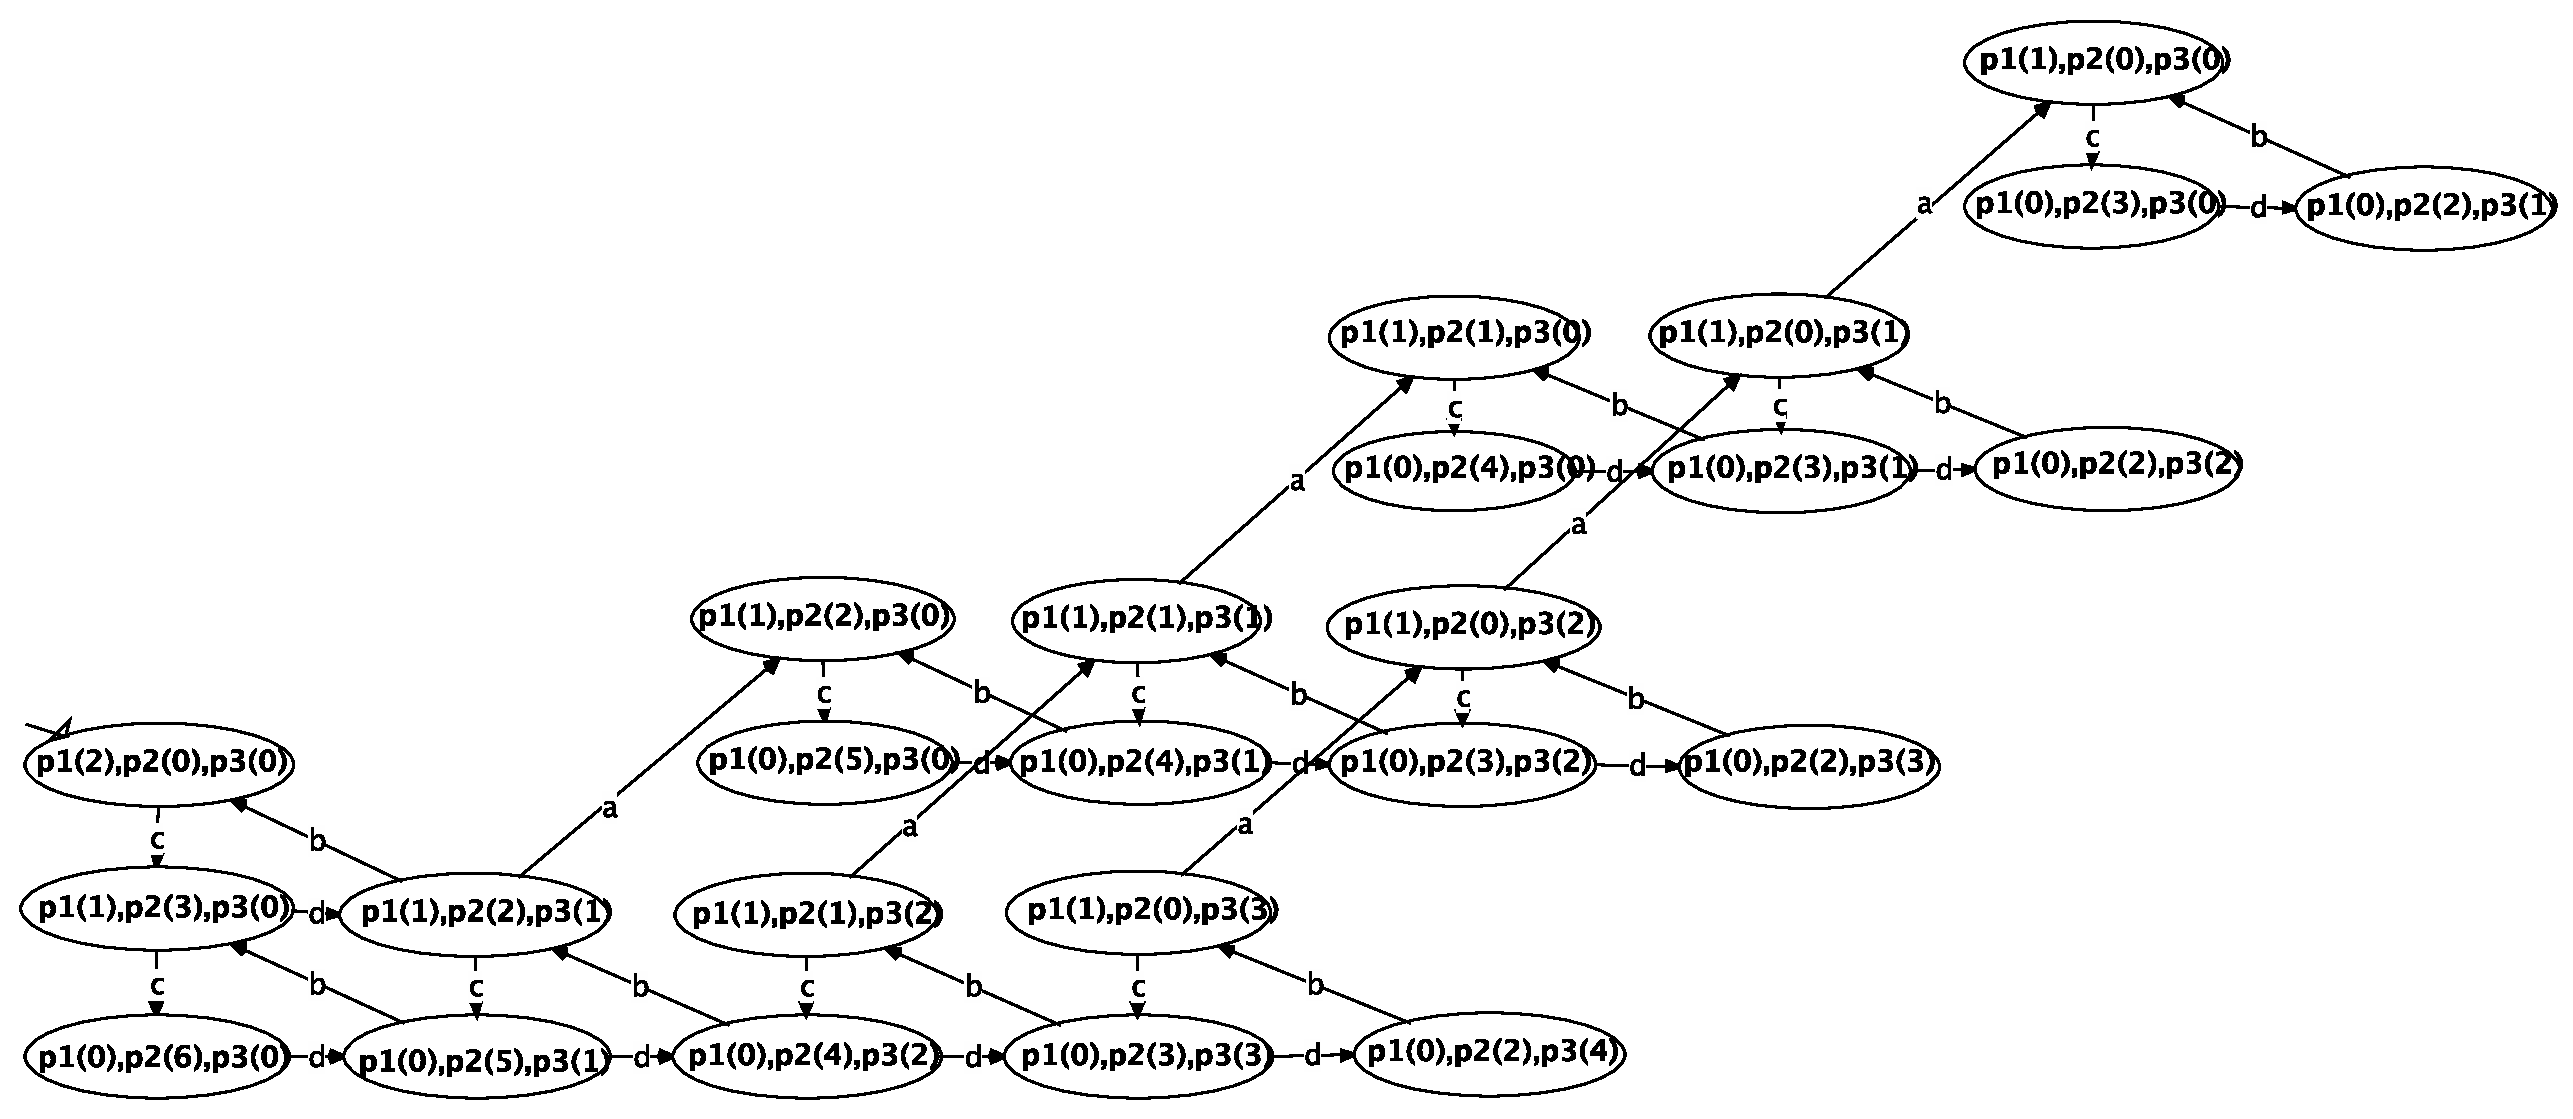
\includegraphics[scale=0.35]{8_4errg.pdf}
	\caption{Erreichbarkeitsgraph von N8.4}
\end{figure}

Davon ausgehend wurden die starken Zusammenhangskomponenten \( C_1, C_2, C_3 \) und \( C_4 \) gebildet:

\begin{figure}[h!]
	\centering
	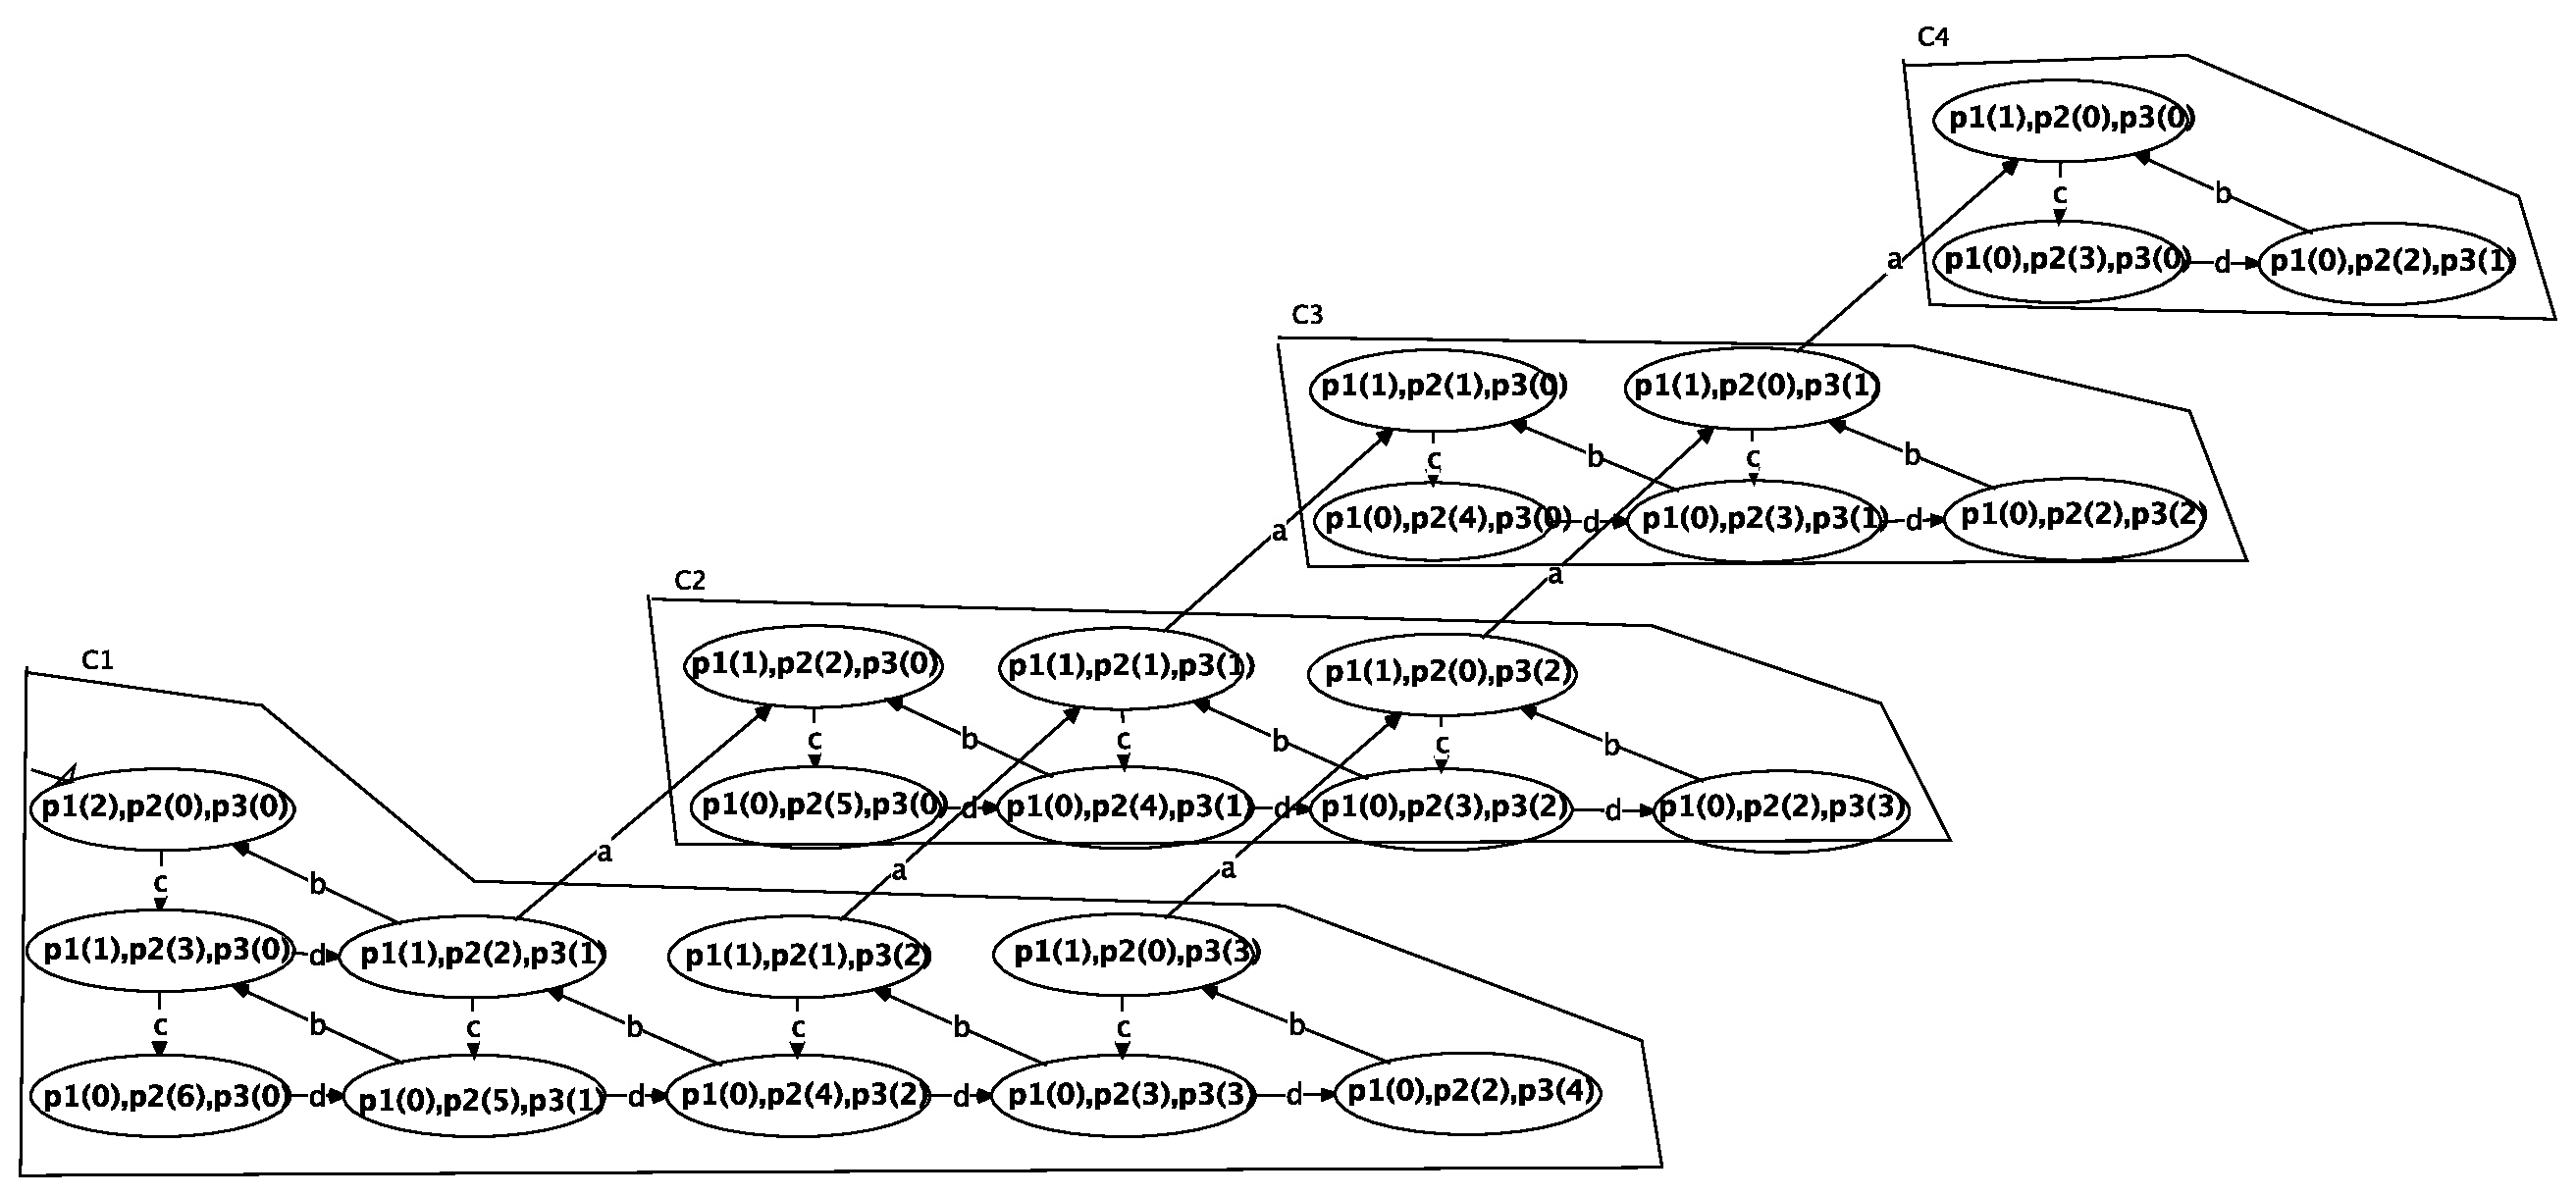
\includegraphics[scale=0.35]{8_4SZK.pdf}
	\caption{SZKs von N8.4}
\end{figure}

Anschließend wurde daraus der reduzierte Graph \(RG^c(\mathcal{N},m_0)\) erstellt.\\
Dabei ist \(V_c = \{C_1,C_2,C_3,C_4\}\) die Knotenmenge, welche von den SZKs gebildet wird und\\
\(E_c = \{(C_1,a,C_2), (C_2,a,C_3), (C_3,a,C_4)\}\) die Kantenmenge.

\begin{figure}[h!]
	\centering
	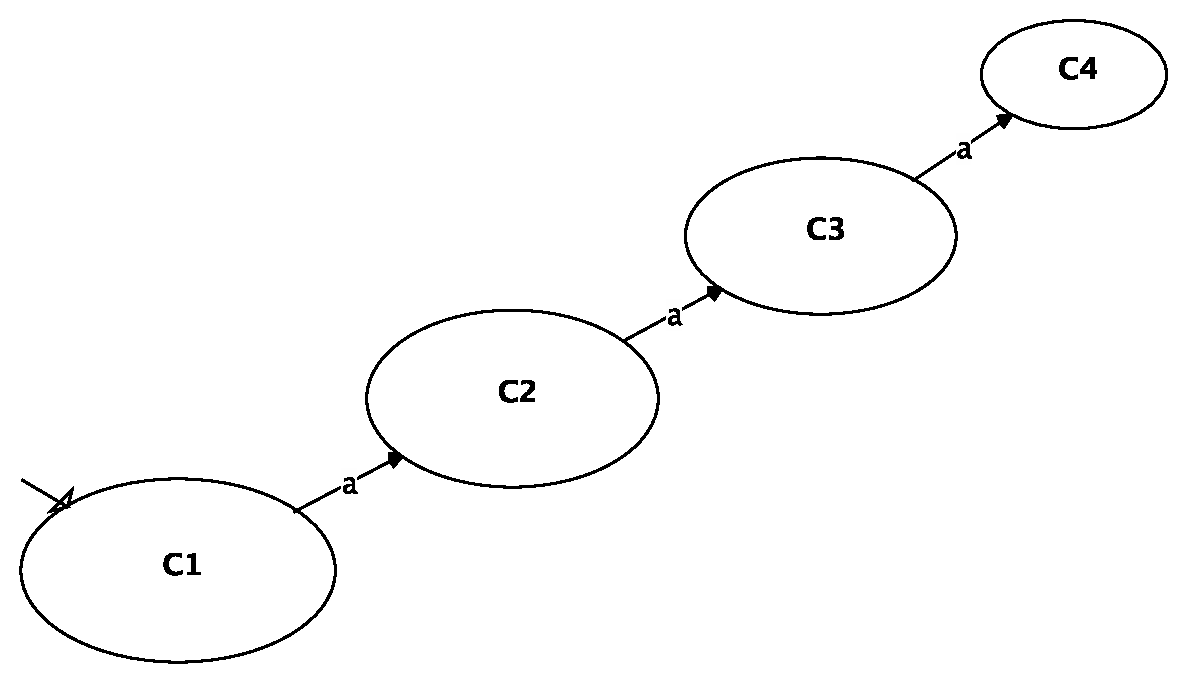
\includegraphics[scale=0.4]{8_4RGc.pdf}
	\caption{reduzierter Graph von N8.4}
\end{figure}

Von den Zusammenhangskomponenten ist \(C_4\) terminal, d.h. \(F=\{C_4\}\).\\
Da nur $C_{4}$ terminal ist und lediglich drei Markierungen enthält, müssen im folgenden auch nur diese betrachtet werden.\\
In der Markierung $m_{1}=p_{1}(1),p_{2}(0),p_{3}(0)$ ist die Transition $c$ aktivierbar,
in der Markierung $m_{1}=p_{1}(0),p_{2}(3),p_{3}(0)$ ist die Transition $d$ aktivierbar und in der Markierung $m_{1}=p_{1}(0),p_{2}(2),p_{3}(1)$ ist die Transition $b$ aktivierbar. Für diese drei Transitionen gibt es im Umkehrschluss also eine Markierung in der sie aktivierbar sind. Der Algorithmus bestimmt die Transitionen $b$, $c$, $d$ folglich als lebendig. Für die Transition $a$ gibt es keine Markierung in $C_{4}$ in der sie aktivierbar wäre. Folglich ist sie nicht lebendig.


\section*{Aufgabe 8.5}
\subsection*{1.}
Das in Abbildung 7 gezeigte Netz simuliert eine Lieferung per Drohne. Dabei stellt die Transition $t_1$ die Bestellung dar, die in Form von Marken festgehalten werden. Von Transition $t_2$ werden diese Marken entfernt (Abholung) und auf den nächsten Platz gelegt. Der nächste Schritt ist die Auslieferung des Pakets. Dies wird durch eine Entfernung einer Marke aus dem Drohnen Lager und eines abgeholten Pakets durch Transition $t_3$ simuliert. Das Entfernen der Marke vom letzten Platz durch Transition $t_4$, modelliert den Rückflug der Drohne. Im Lager entsteht entsprechend eine neue Marke.\\

\begin{figure}[h!]
	\centering
	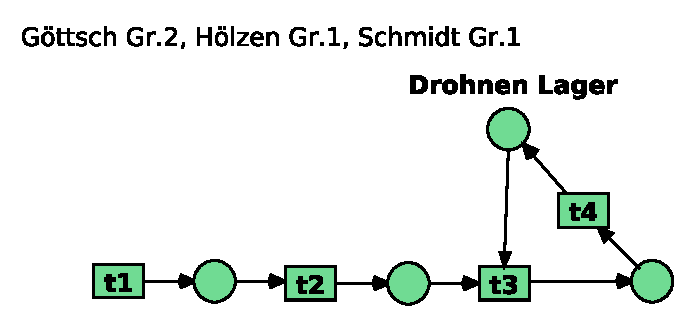
\includegraphics[scale=0.8]{8-5-1.pdf}
	\caption{Erste Simulation}
\end{figure}

\subsection*{2.}
?

\subsection*{3.}
In diesem Netz ist die Anzahl der Marken im Drohnen Lager auf 5 beschränkt.\\

\begin{figure}[h!]
	\centering
	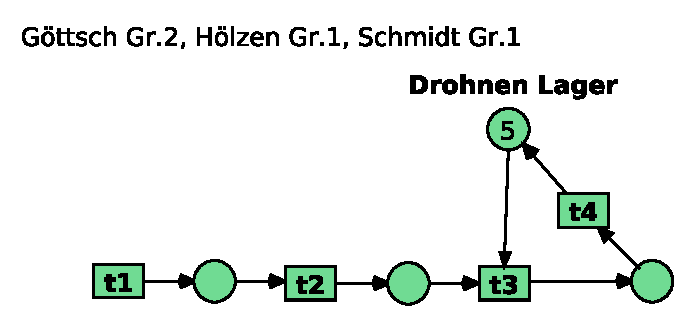
\includegraphics[scale=0.8]{8-5-3.pdf}
	\caption{Erste Simulation}
\end{figure}

\subsection*{4.}
Die Transition $t_5$ markiert defekte Drohnen als auszutauschend, $t_6$ legt eine neue Marke auf das Drohnen Lager, die eine intakte Drohne symbolisiert. Die Kapazität wird hierbei nicht überschritten, es kann jedoch der Fall auftreten, dass alle Drohnen defekt sind und keine Lieferung ausgetragen werden kann.\\

\begin{figure}[h!]
	\centering
	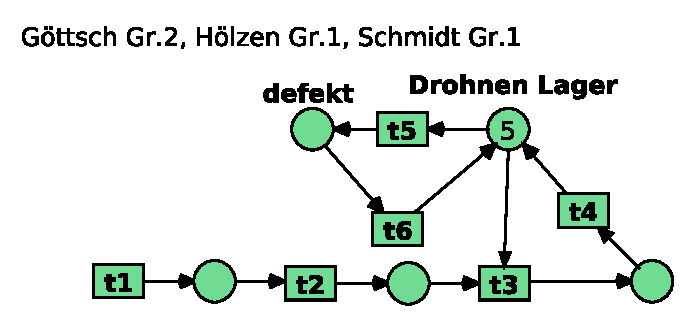
\includegraphics[scale=0.8]{8-5-4.pdf}
	\caption{Erste Simulation}
\end{figure}

\newpage
\subsection*{5.}
Die Transition $t_7$ bzw. die von ihr generierten Marken modellieren einen Abholauftrag. Eine Drohne kann mit $t_8$ zu einem Kunden fliegen und anschließend, indem durch Transition $t_9$ die Drohne mitsamt der Retour vom Platz entfernt werden, zurück zum Lager fliegen.\\

\begin{figure}[h!]
	\centering
	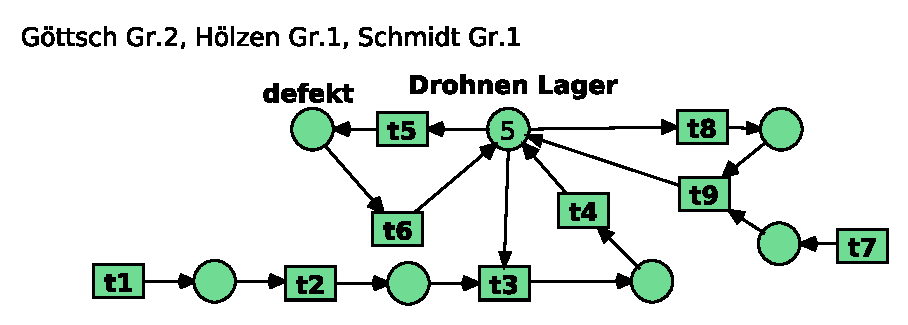
\includegraphics[scale=0.8]{8-5-5.pdf}
	\caption{Erste Simulation}
\end{figure}

\end{document}
